\chapter{Generelle Reflexion}
Das folgende Kapitel stellt meine Reflexion zum Thema Supply Chain Management in Verbindung mit dem SAP System, insbesondere der SAP \ac{APO} Komponente dar. Die Reflexion gliedert sich in die Abschnitte Voraussetzungen, Alternative und mögliche Lösung. Jeder Abschnitt beginnt mit einer Fragestellung und versucht im Anschluss diese zu beantworten.
Die Reflexion beginnt mit dem Ziel und den \textbf{Herausforderungen} eines \ac{SCM}. Beim Abschnitt \textbf{Voraussetzungen} soll kurz ein zentralistischer \ac{SCM} Ansatz betrachtet werden. Im Abschnitt \textbf{Alternativen} sollen kurz die möglichen Alternativen zu einem zentralistischen Ansatz betrachtet werden und abschließend soll eine mögliche IT-Lösung für das \ac{SCM} beschrieben werden.

\section{Ziele und Herausforderungen des SCM}
Wie in dem vorherigen Kapitel bereits erwähnt, stellt die Planung und Abbildung von komplexen Produktions- und Lieferprozessen diverse Unternehmen vor unterschiedlich große Herausforderungen. Eine der größeren Probleme ist die Planung, die die gesamte Wertschöpfungs- und Lieferkette berücksichtigt. Besonders wenn Abteilungsgrenzen oder unterschiedliche inkompatible Datensätze vorhanden sind, erschwert das die integrierte Planung.
Die Ziele und Aufgaben einer \ac{SCM} werden daher breiter gefasst:
\begin{itemize}
	\item Verkürzung der Liefer- und Durchlaufzeiten
	\item Erhöhung der Termintreue
	\item Kosteneinsparung durch optimierte Bestellmengen und Lagerbestände
	\item Erhöhung der Prognose- und Planungsgenauigkeit
	\item Minimierung von Produktions- und Lieferzeitverzögerungen
	\item Vereinheitlichung von Strategien, beispielsweise für Standortplanung, Produkt- und Lieferantenauswahl
\end{itemize}
Eins der größten Probleme, vor dem viele Unternehmen stehen, ist die Einführung einer \ac{SCM}. Zum einen fehlt das Know-How, zum anderen fehlt es an geeignetem Personal und an der entsprechenden Infrastruktur. Typischerweise wird eine Beratungs- und Implementierungshilfe in Anspruch genommen, die das Unternehmen während der gesamten Einführungsphasen bis zur Inbetriebnahme begleitet. Darüber hinaus müssen die Mitarbeiter des entsprechenden Unternehmens zur Einführung des \ac{SCM} bereit sein. Dazu gehört neben den organisatorischen Voraussetzungen, wie Prozessorientierung und Transparenz auch ein vollumfassender Informationsaustausch.
Das Problem von umfassender \ac{SCM} liegt in den verschwimmenden Grenzen der Abteilungen und Unternehmen. Zum einen wird die Verteilung des erwirtschafteten Gewinns verschleiert, was zu Konflikten mit den \ac{SCM} Partnerunternehmen führt. Zum anderen können \ac{SCM} Partner insolvent werden und durch die verschwommenen Grenzen, lässt sich nicht eindeutig festmachen, wer die anfallenden Kosten tragen muss. Darüber hinaus ergeben sich die folgenden Punkte als weitere Herausforderungen für ein funktionierendes \ac{SCM}:
\begin{itemize}
	\item Ganzheitliche Steuerung und Entscheidungen über multiple Standorte hinweg, wodurch die jeweiligen Standorte an Bedeutung verlieren
	\item Erhöhte Komplexität und Steuerungsaufwand, da unternehmensspezifische Prozesse und Abläufe mit dem Unternehmen gewachsen sind
	\item Unternehmensübergreifenden Prozesse, als Voraussetzung für Änderungen oder Neudefinition von Prozessen
	\item Prozessmodellierung, um bestehende Prozesse effizienter zu gestalten und Optimierungspotenziale zu erkennen
	\item Vollständige Transparenz bei Ressourcen und Kapazitäten, da andernfalls die Planung nicht zentral ausgeführt werden kann. 
	\item Interkompatibilität zwischen den Produktionstechnologien der \ac{SCM}-Partner, da inkompatible Technologien die Flexibilität verringern und Abhängigkeiten verursachen
	\item "`Backpressure"` bei \ac{SCM}-Partner in infrastrukturell schwächeren Gegenden. Das führt zu einer Überlastung bei der Datenübertragung, was zu Verlust von Daten und Informationen führen kann
\end{itemize}

\section{Voraussetzungen für einen zentralistischen Ansatz}
Bei einer ganzheitlichen Lösung die übergreifend für alle Standorte plant, handelt es sich um einen zentralistischen Ansatz des \ac{SCM}.
Dabei befindet sich die \ac{SCM} an einem bestimmten Standort, der Teil der \ac{SC} ist. Dabei sind sämtliche \ac{ERP}-Systeme der \ac{SC} mit dem \ac{SCM} gekoppelt, damit die Bedarfs- und Verfügbarkeitsprüfung über die gesamte Supply Chain erstellt werden kann.
Dabei muss sichergestellt werden, dass die Daten in einem bestimmten Format gesendet und empfangen werden, damit mit diesen Daten sinnvoll weitergearbeitet wird. Wie im vorherigen Kapitel bereits angerissen, nutzt das SAP \ac{ERP} System das Core Interface \cite{scm:cif_10} um zwischen dem SAP \ac{ERP} und SAP \ac{APO} System die Daten auszutauschen.
Werden zusätzlich nicht SAP System angeschlossen, so bietet SAP die Möglichkeit mittels \ac{BAPI}’s eigenen Schnittstellen zu entwickeln und den angeschlossenen Systemen zur Verfügung zu stellen. 
Abseits der Integration der Daten und Definition und Erstellung von Schnittstellen, ist auch die Transparenz ein Problem von zentralistischen Lösungen. Jeder \ac{SCM}-Partner muss seinen Daten für alle freigeben. Dabei müssen die Unternehmen darauf vertrauen, dass kein Missbrauch betrieben wird. Zusätzlich zum Vertrauen spielen auch Sicherheitsaspekte eine übergeordnete Rolle. 
Gerade beim Transfer der Daten über das Internet, muss die Sicherheit und Integrität der Daten gewährleistet werden. Manipulierte Daten liefern keine korrekten Ergebnisse, was sich auf die gesamte \ac{SC} auswirken kann und negativen Einfluss auf die Qualität der Prognose hat. 
Werden nicht SAP System angeschlossen, gehören zusätzlich zur Definition der Daten und Schnittstellen, auch ein Mapping der Daten auf das Zielsystem. Sind die Begrifflichkeiten nicht eindeutig definiert, werden die Daten gegebenenfalls falsch interpretiert und verarbeitet, was sich wiederrum in einer schlechten Qualität wiederspiegelt. Für gewöhnlich werden die Informationen zur Zuordnung vom SAP System bereitgestellt und müssen von den angeschlossenen Systemen importiert und verarbeitet werden (Stichwort: Web-Services mit SOAP und WSDL).
Dadurch das, zum einen die Schnittstellen definiert, die Daten bereitgestellt und zum anderen ein Mapping generiert werden muss, ist die Anbindung weitere Unternehmen mit nicht unerheblichem Aufwand verbunden. Dabei entsteht der Aufwand beim Unternehmen das angebunden werden soll, sowie beim Unternehmen, in das eingebunden wird. Um diesen Aufwand zu rechtfertigen sollte bereits ein längere Beziehung oder Partnerschaft zwischen den Unternehmen bestehen.

\section{Alternativen zum zentralistischen Ansatz}
Wie im vorherigen Abschnitt beschrieben, ist der zentralistische Ansatz mit vielen Einschränkungen und Aufwänden verbunden. Besonders wenn  ein Partner angebunden wird, muss die Produktion und die Strategie des Partners übernommen oder angepasst werden. Dieser Aufwand fällt für jeden neuen Partner, beziehungsweise jedes neue Unternehmen erneut an, da die Strategien nicht pauschal übernommen werden können, und stets angepasst werden müssen.
Eine potentielle Alternative dazu stellt das Konsignationslager \cite[vgl. mit]{wiki:konsig_17_11} dar. Wie in \ref{fig:desc_netzwerk} zu sehen ist, werden diese Lager, von ein oder mehrere \ac{SCM}-Partnern, in der Nähe zum Kunden betrieben.

\begin{figure}[htbp]
	\centering
	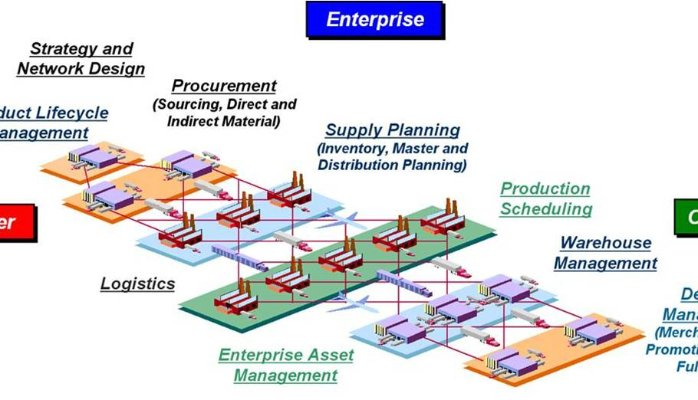
\includegraphics[width=0.8\textwidth]{../pics/scm_komponent}
	\caption{Dezentrales SC-Netzwerk \cite{scm:grafik_decentr_lager_13}}
	\label{fig:desc_netzwerk}
\end{figure}

Das weiterhin \ac{SC} Teilnehmen verbunden sind, kann durch diese die Informationsverarbeitung durchgeführt und an alle Beteiligte verteilt werden. Dadurch soll, bei unerwarteten Ausfällen innerhalb der \ac{SC}, das System alle nötigen Informationen an die Beteiligten weiterleiten, damit diese die Produktionsplanung entsprechend anpassen können.
Wichtig bei dezentralen Systemen ist, dass sich alle beteiligten Systeme dynamisch an die geänderte Situation anpassen und entsprechenden reagieren können. Dazu gehört, dass auch die Planung, Verwaltung und Steuerung der Ressourcen schnell angepasst werden können. Dabei dürfen die Konditionen bezüglich der Liefertermine, Mengen und Qualität nicht vernachlässigt werden.
Die Abbildung 4 zeigt den Prozess mit einem Konsignationslager beim Kunden. Das Lager des Kunden wird vom Lieferanten befüllt. Sobald der Kunde ein Bedarf für ein Produkt erkennt, entnimmt er es aus dem Konsignationslager. Dabei wird ein Warenausgang gebucht und der Lieferant wird darüber informiert. Anschließend stellt dieser eine Rechnung an den Kunden und befüllt das Lager erneut.
Der Vorteil bei diesem Vorgang, ist das dem Kunden der genaue Bedarf und der Zeitpunkt, an dem er gebraucht wird nicht bekannt sein müssen. Der Lieferant hingegeben hat den Vorteil, dass er sich seine Produktionskapazitäten frei einteilen kann. Er muss lediglich sicherstellen, dass sich im Konsignationslager beim Kunden stets ausreichend Teile befinden. Zusätzlich muss nicht das gesamte System an das \ac{SCM} angeschlossen sein. Das hat insbesondere dann den Vorteil, wenn die Partner sich nicht lange kennen, zwischen ihnen noch keine Partnerschaft besteht oder der Aufwand für die Einführung eines \ac{SCM} als zu groß angesehen wird.

\begin{figure}[htbp]
	\centering
	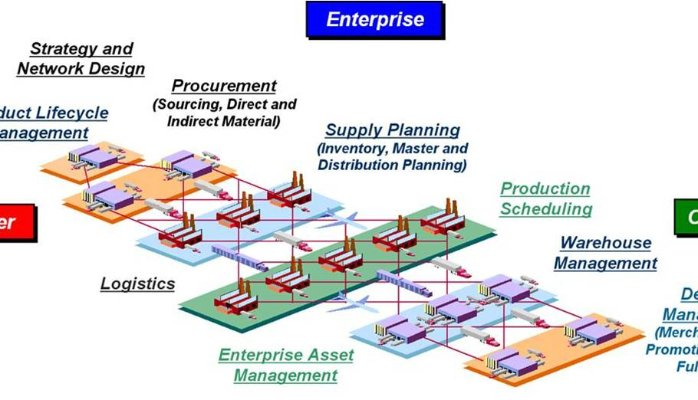
\includegraphics[width=0.8\textwidth]{../pics/scm_komponent}
	\caption{Prozess mit Konsignationslager beim Kunden \cite{scm:grafik_kons_best_kunde_14}}
	\label{fig:kons_prz_kunde}
\end{figure}

\section{Möglich Lösung}
Für eine mögliche IT Umsetzung eines \ac{SCM} Systems bietet sich Web-basierte Lösung an. Die \ac{SCM} wird als REST-Service bereitgestellt und ermöglicht den Unternehmen, sich mit ihren Produkten oder Komponenten anzumelden und sie anderen Teilnehmern zum Erwerb anzubieten. Analog zu einem Marktplatz, können die Teilnehmer nach den benötigten Produkten suchen, bei dem Unternehmen anfragen und entsprechend bestellen. Sind beim Unternehmen ausreichend freie Kapazitäten vorhanden, produziert und verschickt das Unternehmen das Produkt an den Besteller. 
Der Vorteil bei diesem Vorgehen ist die Trennung der festen Bindung zwischen Kunde und Unternehmen, womit auch kein Datenaustausch und standardisierte Schnittstellen benötigt werden.

